\documentclass[usenames,dvipsnames,aspectratio=169]{beamer}
    \mode<presentation> {
    \usetheme{Montpellier}
    \useoutertheme{tree}
    \usecolortheme{beaver}
    %\setbeamertemplate{footline} % To remove the footer line in all slides uncomment this line
    \setbeamertemplate{footline}[page number] % To replace the footer line in all slides with a simple slide count uncomment this line
    \setbeamertemplate{navigation symbols}{} % To remove the navigation symbols from the bottom of all slides uncomment this line
    \setbeamersize{text margin left=8mm,text margin right=5mm}
    }

    \usepackage{graphicx} % Allows including images
    \usepackage{booktabs} % Allows the use of \toprule, \midrule and \bottomrule in tables
    \usepackage{minted}
    \usepackage{xcolor}
    \usepackage[utf8]{inputenc}
    \usepackage{pifont}
    \usepackage{xspace}
    \usepackage{newunicodechar}
    \usepackage{hyperref}

    \usepackage[pdf]{graphviz}

    \newunicodechar{✪}{\ding{74}}

    \definecolor{mintedbackground}{rgb}{0.95,0.95,0.95}
    \newcommand{\code}[1]{\colorbox{lightgray}{\texttt{#1}}}
    \newcommand{\distage}{\texttt{distage}\xspace}

\newminted{scala}{
    bgcolor=mintedbackground,
    fontfamily=tt,
    linenos=true,
    numberblanklines=true,
    numbersep=5pt,
    gobble=0,
    frame=leftline,
    framerule=0.4pt,
    framesep=2mm,
    funcnamehighlighting=true,
    tabsize=4,
    obeytabs=false,
    mathescape=false
    samepage=false, %with this setting you can force the list to appear on the same page
    showspaces=false,
    showtabs =false,
    texcl=false,
}

\newminted{text}{
    bgcolor=mintedbackground,
    fontfamily=tt,
    linenos=true,
    numberblanklines=true,
    numbersep=5pt,
    gobble=0,
    frame=leftline,
    framerule=0.4pt,
    framesep=2mm,
    funcnamehighlighting=true,
    tabsize=4,
    obeytabs=false,
    mathescape=false
    samepage=false, %with this setting you can force the list to appear on the same page
    showspaces=false,
    showtabs =false,
    texcl=false,
}

\newminted{json}{
    bgcolor=mintedbackground,
    fontfamily=tt,
    linenos=true,
    numberblanklines=true,
    numbersep=5pt,
    gobble=0,
    frame=leftline,
    framerule=0.4pt,
    framesep=2mm,
    funcnamehighlighting=true,
    tabsize=4,
    obeytabs=false,
    mathescape=false
    samepage=false, %with this setting you can force the list to appear on the same page
    showspaces=false,
    showtabs =false,
    texcl=false,
}

    \setminted{fontsize=\footnotesize,baselinestretch=1}

    \usepackage{tikz}
    \usetikzlibrary{positioning}
    \graphicspath{{target/media/}}

    \title{Hyperpragmatic pure FP testing with distage-testkit}

    \institute[Septimal Mind Ltd]
    {
    Septimal Mind Ltd\\
    \medskip
    \textit{team@7mind.io}
    }
    \date{\today}


\makeatletter
\setbeamertemplate{headline}
{%
    \begin{beamercolorbox}[wd=\paperwidth,colsep=1.5pt]{upper separation line head}
    \end{beamercolorbox}
    \begin{beamercolorbox}[wd=\paperwidth,ht=2.5ex,dp=1.125ex,%
      leftskip=.3cm,rightskip=.3cm plus1fil]{title in head/foot}
      \usebeamerfont{title in head/foot}\insertshorttitle
    \end{beamercolorbox}
    \begin{beamercolorbox}[wd=\paperwidth,ht=2.5ex,dp=1.125ex,%
      leftskip=.3cm,rightskip=.3cm plus1fil]{section in head/foot}
      \usebeamerfont{section in head/foot}%
      \ifbeamer@tree@showhooks
        \setbox\beamer@tempbox=\hbox{\insertsectionhead}%
        \ifdim\wd\beamer@tempbox>1pt%
          \hskip2pt\raise1.9pt\hbox{\vrule width0.4pt height1.875ex\vrule width 5pt height0.4pt}%
          \hskip1pt%
        \fi%
      \else%
        \hskip6pt%
      \fi%
      \insertsectionhead
      \usebeamerfont{subsection in head/foot}%
      \ifbeamer@tree@showhooks
        \setbox\beamer@tempbox=\hbox{\insertsubsectionhead}%
        \ifdim\wd\beamer@tempbox>1pt%
          \ \raise1.9pt\hbox{\vrule width 5pt height0.4pt}%
          \hskip1pt%
        \fi%
      \else%
        \hskip12pt%
      \fi%
      \insertsubsectionhead\hfill\insertframenumber/\inserttotalframenumber\hspace{0.5em}
    \end{beamercolorbox}
    \begin{beamercolorbox}[wd=\paperwidth,colsep=1.5pt]{lower separation line head}
    \end{beamercolorbox}
}
\makeatother

\begin{document}

\begin{frame}
%\titlepage

\begin{figure}
\color{RubineRed}
\Huge Hyperpragmatic pure FP testing \\
with \\
distage-testkit

\rule{\linewidth}{1mm}

\normalsize Functional Scala 2019
\end{figure}

\begin{figure}
  Septimal Mind Ltd \\
  \textit{team@7mind.io} \\
  
\includegraphics[width=0.2\textwidth]{media/logo_7mind.png}
\end{figure}

\end{frame}

%%%%%%%%%%%%%%%%%%%%%%%%%%%%%%%%%%%%%%%%%%%%%%%%%%%%%%%%%%%%%%%%%%%%%%%%%%%%%%%%%%%%%%%%%%%%%%%%%%%
\section{Tests and Test Taxonomies}

\begin{frame}
  \frametitle{Not all the tests are equal}

  \begin{figure}
  \Large
  Tests are important. We know that. \\
  Tests are the simplest way to define and verify important contracts. \\
  And contracts are crucial for project maintainability and viability. \\
  \Huge We write tests. A lot of. \\
  \end{figure}

  \begin{figure}
  \Large
  But \\
  \dots \\
  some tests prove themselves useful and some do not.
  \end{figure}
\end{frame}

\begin{frame}
  \frametitle{Not all the tests are equal}

  \begin{figure}
  \Huge Which tests are good and which are bad?
  \end{figure}
\end{frame}

\begin{frame}
  \frametitle{Bad test criterias}

  Bad tests are:
  \begin{itemize}
    \item \textbf{Slow},
    \item \textbf{Unstable}: they fail randomly,
    \item \textbf{Nonviable}: they don’t survive refactorings,
    \item \textbf{Demanding}: they require complex preconditions to be met: external services up and running, fixtures loaded, etc, etc,
    \item \textbf{Incomprehensible}: they signal about a problem but don’t help us to localize the cause.
  \end{itemize}
\end{frame}

\begin{frame}
  \begin{figure}
  \Huge We spend more resources to write and maintain bad tests \\
  than the value they bring us.
  \end{figure}
\end{frame}

\begin{frame}
  \begin{figure}
  \Huge How may we make our tests better?
  \end{figure}
\end{frame}

\begin{frame}
  \begin{figure}
  \Large Let's ditch Unit/Functional/Integration trinity\dots \\
  \Huge \dots and introduce some new terminology
  \end{figure}
\end{frame}

\begin{frame}
  \frametitle{Test Taxonomy: Encapsulation Axis}
  Let's say that every test falls under one of the following categories:

  \begin{enumerate}
    \item \textbf{Blackbox} tests check just interfaces not knowing anything about implementations behind them,
    %%\item \textbf{Effectual} tests use only interfaces, but also verify some side-effects (a file created on the disk) which cannot be, or are hard to explicitly express.
    \item \textbf{Whitebox} tests may know about implementations and check them directly, sometimes even breaking into some internal state to verify if it conforms to test expectations.
  \end{enumerate}
\end{frame}

\begin{frame}
  \frametitle{Test Taxonomy: Isolation Axis}
  Let's say that every test falls under one of the following categories:

  \begin{itemize}
    \item \textbf{Atomic} tests check just one ``unsplittable'' software component,
    \item \textbf{Group} tests check multiple software components,
    \item \textbf{Communication} tests communicate with outer world (databases, API providers, etc, etc).
  \end{itemize}
\end{frame}

\begin{frame}
  \begin{figure}
  \large You may extend and modify this Test Taxonomy as it would be convenient for you.
  \end{figure}

  \begin{figure}
    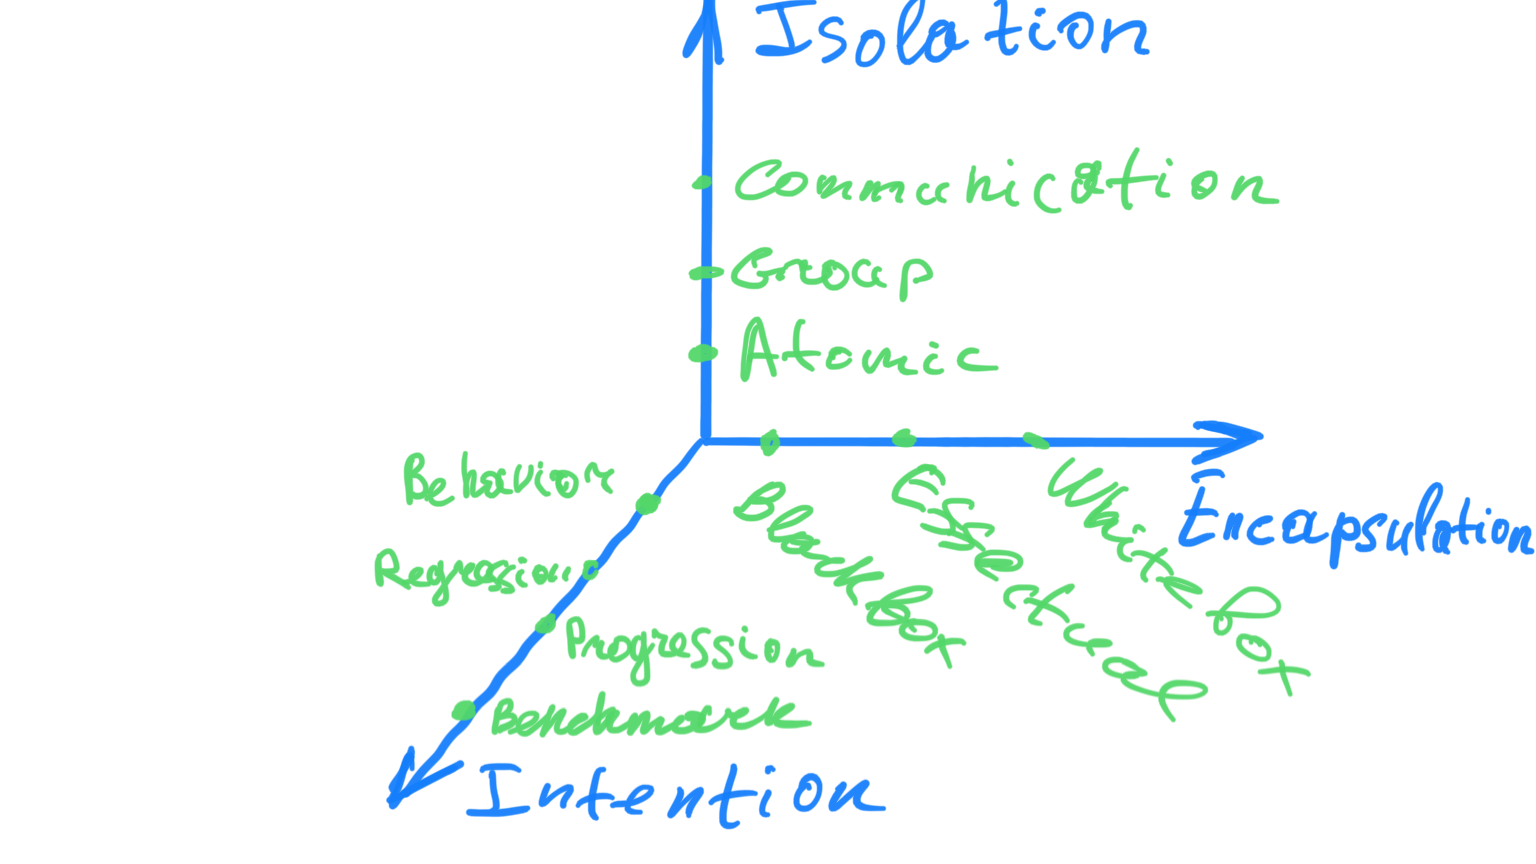
\includegraphics[width=0.7\textwidth]{media/ctt.png}
  \end{figure}

  \begin{figure}
  More about test taxonomies: \url{https://blog.7mind.io/constructive-test-taxonomy.html}
  \end{figure}
\end{frame}


\begin{frame}
  \frametitle{Test Taxonomy: Why So?}
  \begin{figure}
    According to our experience the best tests are \\
     \textbf{Blackbox} tests with \textbf{Atomic} or \textbf{Group} Isolation Level.
  \end{figure}
  \begin{figure}
    This makes sense: such tests are fast and refactßoring-resilient.
  \end{figure}
\end{frame}

\begin{frame}
  \frametitle{Communication tests}
  But in real projects most of the tests fall under \textbf{Communication} category  (``Integration'' tests).

  \vspace{0.3cm}
  Why?
  \begin{enumerate}
  \item Engineers want to test The Whole Thing,
  \item It's hard to separate components,
  \item etc, etc\dots
  \end{enumerate}
\end{frame}

\begin{frame}
  \frametitle{Communication tests can be more useful}

  \begin{figure}
  We may replace \textit{integration components} with \textit{Dummies}\footnotemark[1].
  \end{figure}

  \begin{figure}
  This way we may turn \\
  \textbf{Communication} tests \\
  into \\
  \textbf{Group} or \textbf{Atomic}\footnotemark[2]
  \end{figure}

  \footnotetext[1]{people also call them \textit{``Fakes''}, \textit{``in-memory implementations''} or \textit{``Mocks''}}
  \footnotetext[2]{this statement is valid for \textbf{Blackbox} tests only}
\end{frame}


\section{Dual Test Tactic}
\begin{frame}
  \frametitle{Dual Test Tactic}
  The same test scenario executed with both Production and Dummy implementations of \textit{integration components} is beneficial:

  \begin{enumerate}
  \item We can test business logic quickly, without any interference,
  \item We still able to verify business logic behaviour with ``real'' integrations,
  \item \textbf{Dual Test Tactic} enforces us to follow \textbf{LSP} and design better.
  \end{enumerate}

  \begin{figure}
  Refactorings are crucial for long-term health of the project. \\
  \textbf{Blackbox} tests enable refactorings. \\
  \textbf{Dual Test Tactic} drastically reduces the price of refactorings.
  \end{figure}
\end{frame}

\begin{frame}
  \frametitle{Dual Test Tactic: ideas}

  \begin{enumerate}
    \item \underline{Ignore} \textbf{Communication} tests in case their dependencies are unsatisfied (service unavailable), don't fail,
    \item \underline{Avoid} automatic \textit{``Mocks''}, they prevent encapsulation,
    \item \underline{Never run} heavy dependencies in-process
    \begin{itemize}
      \item don't bring whole Kafka or Cassandra into the classpath. \textbf{PLEASE}
    \end{itemize}
  \end{enumerate}
\end{frame}

\begin{frame}
  \frametitle{Dual Test Tactic: The Main Issue}

  \begin{figure}
  It's easy to setup test dependencies while working with \textit{Dummies} \\
  But you have to do things differently for \textit{Production} dependencies.
  \end{figure}

  We have to take care of:
  \begin{enumerate}
    \item Resource acquisition and Cleanups,
    \item Speed,
    \item Memoization and resource reuse,
    \item Interference,
    \item \dots
  \end{enumerate}
\end{frame}

\begin{frame}
  \frametitle{Dual Test Tactic: dummy repositories testcase}
  \begin{figure}
  \digraph[scale=0.7]{dummytestplan}{
      node  [style="rounded,filled,bold", shape=box, width=1.3]
      r1 [label="make[UserRepo]", color=darkolivegreen1];
      r2 [label="make[AccountsRepo]", color=darkolivegreen1];
      s1 [label="make[UserService]", color=darkolivegreen1];
      s2 [label="make[AccountsService]", color=darkolivegreen1];
      t1 [label="run[MyTestCase]", color=cadetblue1];
      t2 [label="run[AnotherTestCase]", color=cadetblue1];
      r1 -> s1 -> t1;
      r2 -> s2 -> t1;
      s1 -> t2;
      s2 -> t2;
   }
   \end{figure}
\end{frame}

\begin{frame}
  \frametitle{Dual Test Tactic: production repositories testcase}

  \begin{columns}
  \begin{column}[T]{0.4\textwidth}
    \setlength{\topsep}{0pt}
    \setlength{\partopsep}{0pt}

    \vspace{-1.22cm}
    \begin{figure}
    %\hspace*{-1.65cm}
    \digraph[scale=0.42]{prodtestplan}{
        graph [pad="0.2", nodesep="0.2", ranksep="0.2"];
        splines="false";
        node  [style="rounded,filled,bold", shape=box, width=1.3];
        dbchk [label="probe database port", color=gold];
        db1 [label="make[DbDriver]", color=darkgoldenrod1];
        dbtUsers [label="setup users table", color=darksalmon];
        dbtAccounts [label="setup accounts table", color=darksalmon];
        dbtcUsers [label="remove users table", color=darksalmon];
        dbtcAccounts [label="remove accounts table", color=darksalmon];
        dbdc [label="close driver", color=darkgoldenrod1];
        r1 [label="make[UserRepo]", color=darkolivegreen1];
        r2 [label="make[AccountsRepo]", color=darkolivegreen1];
        s1 [label="make[UserService]", color=darkolivegreen1];
        s2 [label="make[AccountsService]", color=darkolivegreen1];
        t1 [label="run[MyTestCase]", color=cadetblue1];
        t2 [label="run[AnotherTestCase]", color=cadetblue1];
    subgraph cluster_0 {
        label="Setup";
        labeljust="l";
        dbchk -> db1;
        db1 -> dbtUsers;
        db1 -> dbtAccounts;
        dbtUsers -> r1 -> s1;
        dbtAccounts -> r2 -> s2;
      }
    subgraph cluster_1 {
        label="Execute";
        labeljust="l";
        s1 -> t1;
        s2 -> t1;
        s1 -> t2;
        s2 -> t2;
    }
    subgraph cluster_2 {
        label="Cleanup";
        labeljust="l";
        t1 -> dbtcUsers;
        t2 -> dbtcUsers;
        t1 -> dbtcAccounts;
        t2 -> dbtcAccounts;
        dbtcAccounts -> dbdc;
        dbtcUsers -> dbdc;
    }
    }
    \end{figure}
  \end{column}

  \begin{column}[T]{0.6\textwidth}
  \vspace{-0.3cm}
  \begin{enumerate}
  \item Order
  \item How to avoid unneccessary job?
    \begin{enumerate}
    \item Memoize resources?..
    \item In a singleton?..
    \item When we close resources?..
    \item On JVM shutdown?.. Oops, SBT\dots
    \item Disambiguation (same class, different parameters)?..
    \end{enumerate}
  \item Resource deallocation
    \begin{enumerate}
    \item \dots even after a failure
    \item Order!
    \end{enumerate}
  \item Other integrations, e.g. run Dockers
    \begin{enumerate}
      \item \dots and await until they open ports
      \item \dots and stop them after the tests
    \end{enumerate}
  \item Configs
  \end{enumerate}
  \end{column}
  \end{columns}


\end{frame}

\begin{frame}
  \frametitle{Dual Test Tactic: Real testcase steps}

  \begin{itemize}
  \item Integration points stack together
  \item \dots and make the problem notably hard

  \item Manual wiring is hard to maintain
  \item \dots and suffers from combinatoric explosion of possible code paths
  \item Cake pattern doesn't make much difference
  \item Conventional DI frameworks fail
  \end{itemize}

  \begin{figure}
  \Large It's hard to setup variable contexts.
  \end{figure}
\end{frame}

\begin{frame}
  \begin{figure}
  \Huge Dual Test Tactic
  \end{figure}

  \begin{figure}
  \LARGE may be very pricy under usual circumstances.
  \end{figure}
\end{frame}

\begin{frame}
  \begin{figure}
  \Huge Can we make it cheap?           
  \end{figure}
\end{frame}

\begin{frame}
  \begin{figure}
  \Huge Yes.
  \end{figure}
\end{frame}


\begin{frame}[fragile]
\frametitle{The Goal}

We want to write code like this and never care about setting things up:

\begin{scalacode}
class JustATest[F[+_, +_]] {
  "service" must {
    "do something" in {
      (users: UserService[F], accounts: AccountingService[F]) =>
      for {
        user  <- users.create()
        balance <- accounts.getBalance(user)
      } yield {
        assert(balance == 0)
      }
    }
  }
}

object JustATestZioProd extends JustATest[zio.IO] with Prod
object JustATestZioDummy extends JustATest[zio.IO] with Dummy
\end{scalacode}
\end{frame}

\begin{frame}
  \begin{figure}
  \Huge \color{RubineRed} dist✪ge
  \end{figure}

  \begin{figure}
  \LARGE is a Dependency Injection mechanism for Scala
  \end{figure}

  \begin{figure}
  \large But it lacks negative traits of a typical DI thingy\dots \\
  \Large \dots and has many unique properties. \\
  \dots and it's blazing fast.
  \end{figure}

  \begin{figure}
  \large You may call it a module system for Scala\dots \\
  \Large \dots with automatic garbage-collecting solver
  \end{figure}
\end{frame}

\begin{frame}
  \frametitle{\distage}
  \begin{enumerate}
    \item Supports FP, wires Resources, Effects, ZIO Environments\dots
    \item transparent and predictable
      \begin{itemize}
        \item first plan then do
        \item test the outcome without effect execution!
        \item compile-time checks and tests
      \end{itemize}
    \item no \texttt{scala-reflect} nor Java reflection\footnotemark[1],
      \begin{itemize}
        \item ScalaJS support is coming
      \end{itemize}
    \item is non-invasive.
      \begin{itemize}
        \item You can add it to your project keeping business logic intact\dots
        \item \dots and remove it.
      \end{itemize}
    \item is not an ad-hoc thing, it has strong theory behind.
  \footnotetext[1]{Since version \texttt{0.10.0}, see https://blog.7mind.io/lightweight-reflection.html}
  \end{enumerate}
\end{frame}

\begin{frame}
  \frametitle{Docker support in \distage}

  \begin{figure}
    While we develop and test we may need our integrations up and running\dots \\
    \dots We have \texttt{docker-compose} for that\dots \\
    But manual rituals are annoying and Compose is imperfect \\
    (wait until service opens port? Hah)
  \end{figure}

  \begin{figure}
    Container orchestration is not easy. \\
    But\dots \\
    We made a \distage extension allowing to get rid of Compose in most of the cases.
  \end{figure}

  \begin{figure}
    It can run test containers, reuse and shutdown them. \\
    And it can \textbf{await until the service is ready}.
  \end{figure}

\end{frame}

\begin{frame}
  \begin{figure}
  \Huge Let's look at a \underline{real} example\dots
  \end{figure}

  \begin{figure}
  Source code: https://github.com/7mind/distage-example
  \end{figure}
\end{frame}

% \section{distage}
% \begin{frame}
%   \frametitle{How it works: Plans}
%   \distage takes your bindings and then:
%   \begin{enumerate}
%     \item translates bindings into simple Turing-incomplete DSL (like \code{make}, \code{reference}, etc.),
%     \item represents the DSL statements as Directed Acyclic Graph using dependecy information and breaking circular dependencies if any,
%     \item resolves conflicts (one DAG node with several associated operations),
%     \item performs Garbage Collection (yeah, real one),
%     \item applies other transformations (like config reference resolution),
%     \item turns the DAG back into sequential form --- a Plan --- with topological sorting.
%     \item $\Rightarrow$ the Plan may be introspected, printed, executed in compile-time by a code generator or executed in runtime.
%   \end{enumerate}
% \end{frame}

\begin{frame}
  \begin{figure}
    \huge \distage performs optimal ahead of time planning.
    \\
    It doesn't  do any unnecessary job.
  \end{figure}
\end{frame}

\begin{frame}
  \frametitle{One More Thing: Roles}
  \distage allow you to fuse microservices into ``flexible monoliths''.

  \vspace{0.3cm}
  We may:
  \begin{enumerate}
  \item Develop services (\textit{Roles}) separately, even in a multirepo,
  \item Build a single Docker image with multiple Roles in it,
  \item Run several Roles within one process
    \begin{itemize}
        \item We define roles we want to start as commandline parameters
    \end{itemize}
  \item $\Rightarrow$ higher computation density, savings on infrastructure,
  \item $\Rightarrow$ \textit{substantial} development simplification
      \begin{itemize}
        \item full environment can be started on a low-end machine
        \item with just one command
    \end{itemize}
  \end{enumerate}
\end{frame}

\begin{frame}
  \begin{figure}
    \texttt{distage-framework} is the most productive way to write \\
    maintainable pure functional applications with ZIO. \\
    (And any other monad)
  \end{figure}
  \begin{figure}
    \texttt{distage-testkit} is the best way to make your tests performant and reliable.
  \end{figure}
  \begin{figure}
    \distage is adopted by several different companies and \\
    tested by two years of production usage.
  \end{figure}
\end{frame}

\begin{frame}
    \frametitle{Thank you for your attention}
    \begin{center}
      distage website: \url{https://izumi.7mind.io}
    \end{center}
    \begin{center}
      \color{RubineRed}
      Septimal Mind is an Irish software consultancy and R\&D Company

      \vspace{0.3cm}
      We're looking for clients, contributors, adopters and colleagues ;)
    \end{center}
    \begin{center}
      Contact: team@7mind.io

      \vspace{0.3cm}
      Github: \url{https://github.com/7mind}

      \vspace{0.3cm}
      Slides: \url{https://github.com/7mind/slides}
    \end{center}
    \begin{center}
      \color{RoyalBlue}
      Follow us on Twitter

      \vspace{0.3cm}
      \url{https://twitter.com/shirshovp}

      \vspace{0.3cm}
      \url{https://twitter.com/kai_nyasha}
    \end{center}
\end{frame}

\end{document}
